% JuliaCon proceedings template
\documentclass{juliacon}
%\usepackage{mathabx}
\usepackage{amsmath}
\usepackage{amssymb}
\usepackage{amsfonts}
\usepackage{lmodern}
\usepackage{fontawesome}


\usepackage{tikz}
\usetikzlibrary{shapes,arrows,calc}
\tikzstyle{block} = [thick, draw, rectangle, rounded corners, fill=blue!20,
                       minimum height=3em, minimum width=6em]
\tikzstyle{action} = [thick, draw, circle, fill=red!10]


\newcommand{\R}{{\mathbb R}}
\newcommand{\N}{{\mathbb N}}
\newcommand{\E}{{\mathbb E}}
\newcommand{\Z}{{\mathbb Z}}
\renewcommand{\P}{{\mathbb P}}
\newcommand{\bbC}{{\mathbb C}}
\newcommand{\cO}{\mathcal{O}}
\newcommand{\cF}{\mathcal{F}}
\newcommand{\cE}{\mathcal{E}}
\newcommand{\cX}{\mathcal{X}}
\newcommand{\cA}{\mathcal{A}}
\newcommand{\cS}{\mathcal{S}}
\newcommand{\cR}{\mathcal{R}}
\newcommand{\cB}{\mathcal{B}}
\newcommand{\cP}{\mathcal{P}}
\newcommand{\cM}{\mathcal{M}}

\newcommand{\tV}{\widetilde{V}}
\newcommand{\tF}{\widetilde{F}}
\newcommand{\tQ}{\widetilde{Q}}

\newcommand{\bw}{\mathbold{w}}

\newcommand{\Inv}{\mathop{\mathrm{Inv}}}
\newcommand{\argmax}{\mathop{\mathrm{argmax}}}
\newcommand{\mean}{\mathop{\mathrm{mean}}}
\newcommand{\diam}{\mathop{\mathrm{diam}}}

\setcounter{page}{1}

\begin{document}

% **************GENERATED FILE, DO NOT EDIT**************

\title{Fast, Elegant, Set-oriented Numerical Analysis using GAIO.jl}

\author[1]{A. Herwig}
\author[1]{O. Junge}
\affil[1]{Technical University Munich}

\keywords{Dynamical Systems}

\hypersetup{
pdftitle = {Fast, Elegant, Set-oriented Numerical Analysis using GAIO.jl},
pdfsubject = {JuliaCon 2022 Proceedings},
pdfauthor = {A. Herwig, O. Junge},
pdfkeywords = {Dynamical Systems},
}



\maketitle

\begin{abstract}

GAIO (Global Analysis of Invariant Objects) is a package for set oriented numerics in dynamical systems. It provides algorithms for discretisation of the Koopman operator among other uses. The Koopman operator has been of much interest in the last decade, since it can be used in order to compute, e.g., almost invariant \cite{almostinvariant}, cyclic \cite{complicatedbehavior} and coherent sets \cite{coherent} (to name just some uses). Originally written in the 90s in C, GAIO has been redesigned in Julia and is concise, while outperforming the original.

\end{abstract}

\section{Introduction}

A dynamical system can be characterised by a set of global asymptotic behavoirs. These include stability, invariance of certain regions of phase space, as well as statistical behavior of "typical" trajectories. Such topological and statistical questions (among others) can be answered using a \emph{set-oriented} approach. 

This paper presents a Julia language implementation of such a set-oriented approach to numerical analysis, encapsulated in the package GAIO.jl. The data structures and the algorithmic interface have been completely redesigned such that the code for the algorithms is very concise and close to their mathematical pseudocode. At the same time, the performance is equal or better than that of the original C and Matlab versions. 

\section{Dynamical Systems, Invariant Sets and Measures}

Consider a continuous map $f : Q \to Q$ on some compact domain $Q \subset \R^d$. We recall some basic notions from dynamical systems literature required for the proceeding example. 

\subsection{Attractors}\label{sec:attractors}

A set $A \subset Q$ in phase space is called \emph{forward invariant} if $f(A) \subset A$, \emph{backward invariant} if $f^{-1}(A) \subset A$ \footnote{$f^{-1}(A)$ denotes the preimage}, and \emph{invariant} if it is both forward and backward invariant. An invariant set is called \emph{attracting} if there exists a neighborhood $U \supset A$ such that for any other neighborhood $V \supset A$ there exists an $N \in \N$ such that the tail $\bigcup_{k \geq N} f^k (U)$ is contained in $V$. 

\begin{defi}
    The maximal invariant set contained in $A$ is the set 
    \begin{equation}
        \Inv (A) = \left\{ x \in A \mid \cO^\pm (x) \subset A \right\},
    \end{equation}
    where $\cO^\pm (x) = \bigcup_{k \in \Z} f^{k}(\left\{ x \right\})$ denotes the \emph{full orbit} of $x$ under $f$. 
\end{defi}

It follows immediately from the definition that $\Inv (A)$ contains all other invariant sets which are contained in $A$. The following proposition is important for its computation. 

\begin{proposition}
    \cite{maxinvset}
    If $A \subset Q$ is forward invariant, then $Inv (A) = \bigcap_{k \geq 0} f^k (A)$. 
\end{proposition}

This leads to a natural Ansatz for approximation by inductively tightening a cover of the maximal invariant set by finite collections of boxes. Specifically, given a partition $\cP$ of $Q$ and a covering $\cB$ of the maximal invariant set by elements of $\cP$:

\begin{enumerate}
    \item Refine $\cP$ into a strictly finer partition $\cP'$ such that $\diam (\cP') \leq \theta \cdot \diam (\cP)$ for some fixed $\theta < 1$. Let $\cB'$ be the (refined) covering of $\cB$. 
    \item Map the covering forward under $f$, i.e. cover $f(\vert\cB'\vert)$ \footnote{$\vert \cB \vert = \bigcup_{B \in \cB} B$} by elements of $\cP$. Intersect this covering with $\cB'$. 
\end{enumerate}

A simple way to partition a hyperractangular domain $Q = \left[ l_1, u_1 \right] \times \ldots \times \left[ l_d, u_d \right]$ is to divide it into an $N_1 \times \ldots \times N_d$ - element grid of boxes. 

Consider the system of ordinary differential equations in $3$ dimensions given by 

\begin{equation}
    \label{eq:ode}
    \begin{split}
        &\dot{x} = ax + cyz \\
        &\dot{y} = dy + bx + hzy \\ 
        &\dot{z} = pz + gxy 
    \end{split}
\end{equation}

where $a,b,c,d,p,f,g,h \in \R$ are parameters \cite{3dattractor}. Let $f$ be the time-$2$ integral of the system, discretized using 20 steps of the standard Runge-Kutta $4$th order method. 

\begin{lstlisting}[language=Julia,label=lst:map]
    const a, b, c, d = 0.2, -0.01, 1.0, -0.4
    const p, g, h = -1.0, -1.0, -1.0

    v((x,y,z)) = @. (a,d,p)*(x,y,z) + 
                        (0,b*x,0) + 
                        (c,h,g)*(y,z,x)*(z,x,y)

    f(x) = rk4_flow_map(v, x, 0.01, 20)
\end{lstlisting}

We discretize the domain $Q = \left[ -5, 5 \right]^3$ into a $2 \times 2 \times 2$ grid. 

\begin{lstlisting}[language=Julia,label=lst:box]
    center = (0., 0., 0.)
    radius = (5., 5., 5.)
    Q = Box(center, radius)
    P = BoxPartition(Q, (2, 2, 2))
\end{lstlisting}

$f$ induces a map $F : 2^\cP \to 2^\cP$ \footnote{$2^S$ denotes the power set of $S$} by the relationship 

\begin{equation}
    F \left( \left\{ B \right\} \right) = 
    %\bigcup_{\substack{
    %    R \in \cP \\ R \cap f(B) \neq \emptyset
    %}} \left\{ R \right\}
    \left\{ R \in \cP \mid R \cap f(B) \neq \emptyset \right\}
\end{equation}

(see Fig. \ref{fig:boxcover}). 

\begin{figure}
    \centering
    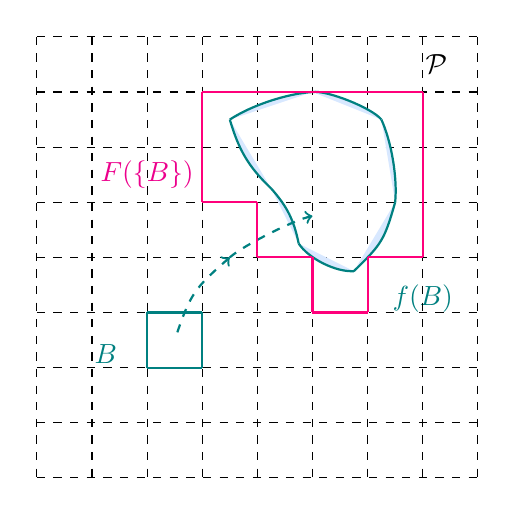
\begin{tikzpicture}[scale=0.7]
    \node [color=black] (0) at (-4, 4) {};
    \node [color=black] (1) at (-3, 4) {};
    \node [color=black] (2) at (-2, 4) {};
    \node [color=black] (3) at (-1, 4) {};
    \node [color=black] (4) at (0, 4) {};
    \node [color=black] (5) at (1, 4) {};
    \node [color=black] (6) at (2, 4) {};
    \node [color=black] (7) at (3, 4) {};
    \node [color=black] (8) at (4, 4) {};
    \node [color=black] (9) at (4, 3) {};
    \node [color=black] (10) at (4, 2) {};
    \node [color=black] (11) at (4, 1) {};
    \node [color=black] (12) at (4, 0) {};
    \node [color=black] (13) at (4, -1) {};
    \node [color=black] (14) at (4, -2) {};
    \node [color=black] (15) at (4, -3) {};
    \node [color=black] (16) at (4, -4) {};
    \node [color=black] (17) at (3, -4) {};
    \node [color=black] (18) at (2, -4) {};
    \node [color=black] (19) at (1, -4) {};
    \node [color=black] (20) at (0, -4) {};
    \node [color=black] (21) at (-1, -4) {};
    \node [color=black] (22) at (-2, -4) {};
    \node [color=black] (23) at (-3, -4) {};
    \node [color=black] (24) at (-4, -4) {};
    \node [color=black] (25) at (-4, -3) {};
    \node [color=black] (26) at (-4, -2) {};
    \node [color=black] (27) at (-4, -1) {};
    \node [color=black] (28) at (-4, 0) {};
    \node [color=black] (29) at (-4, 1) {};
    \node [color=black] (30) at (-4, 2) {};
    \node [color=black] (31) at (-4, 3) {};
    \node [color=black] (32) at (-2, -1) {};
    \node [color=black] (33) at (-1, -1) {};
    \node [color=black] (34) at (-1, -2) {};
    \node [color=black] (35) at (-2, -2) {};
    \node [color=black] (36) at (-2.75, -1.75) {\textcolor{teal}{$B$}};
    \node [color=black] (37) at (-1.5, -1.5) {};
    \node [color=black] (38) at (-0.5, 2.5) {};
    \node [color=black] (39) at (0.25, 1.25) {};
    \node [color=black] (40) at (0.75, 0.25) {};
    \node [color=black] (41) at (1.75, -0.25) {};
    \node [color=black] (42) at (2.5, 1) {};
    \node [color=black] (43) at (2.25, 2.5) {};
    \node [color=black] (44) at (1, 3) {};
    \node [color=black] (45) at (3, -0.75) {\textcolor{teal}{$f(B)$}};
    \node [color=black] (46) at (1, 0.75) {};
    \node [color=black] (47) at (-0.5, 0) {};
    \node [color=black] (48) at (-1, 3) {};
    \node [color=black] (49) at (3, 3) {};
    \node [color=black] (50) at (3, 0) {};
    \node [color=black] (51) at (0, 0) {};
    \node [color=black] (52) at (0, 1) {};
    \node [color=black] (53) at (-1, 1) {};
    \node [color=black] (54) at (2, 0) {};
    \node [color=black] (55) at (1, 0) {};
    \node [color=black] (56) at (1, -1) {};
    \node [color=black] (57) at (2, -1) {};
    \node [color=black] (58) at (-2, 1.5) {};
    \node [color=black] (59) at (-2, 1.5) {\textcolor{magenta}{$F(\{ B \})$}};
    \node [color=black] (60) at (3.25, 3.5) {$\mathcal{P}$};

    \draw [-, dashed] (0.center) to (24.center);
    \draw [-, dashed] (1.center) to (23.center);
    \draw [-, dashed] (2.center) to (22.center);
    \draw [-, dashed] (3.center) to (21.center);
    \draw [-, dashed] (4.center) to (20.center);
    \draw [-, dashed] (5.center) to (19.center);
    \draw [-, dashed] (6.center) to (18.center);
    \draw [-, dashed] (7.center) to (17.center);
    \draw [-, dashed] (8.center) to (16.center);
    \draw [-, dashed] (0.center) to (8.center);
    \draw [-, dashed] (31.center) to (9.center);
    \draw [-, dashed] (30.center) to (10.center);
    \draw [-, dashed] (29.center) to (11.center);
    \draw [-, dashed] (28.center) to (12.center);
    \draw [-, dashed] (27.center) to (13.center);
    \draw [-, dashed] (26.center) to (14.center);
    \draw [-, dashed] (25.center) to (15.center);
    \draw [-, dashed] (24.center) to (16.center);
    \draw [-, draw={rgb,255: red,0; green,128; blue,128}, fill={rgb,255: red,216; green,232; blue,255}, thick] (32.center) to (33.center);
    \draw [-, draw={rgb,255: red,0; green,128; blue,128}, fill={rgb,255: red,216; green,232; blue,255}, thick] (33.center) to (34.center);
    \draw [-, draw={rgb,255: red,0; green,128; blue,128}, fill={rgb,255: red,216; green,232; blue,255}, thick] (34.center) to (35.center);
    \draw [-, draw={rgb,255: red,0; green,128; blue,128}, fill={rgb,255: red,216; green,232; blue,255}, thick] (35.center) to (32.center);
    \draw [-, draw={rgb,255: red,0; green,128; blue,128}, fill={rgb,255: red,216; green,232; blue,255}, thick, bend right=15] (38.center) to (39.center);
    \draw [-, draw={rgb,255: red,0; green,128; blue,128}, fill={rgb,255: red,216; green,232; blue,255}, thick, bend left=15] (39.center) to (40.center);
    \draw [-, draw={rgb,255: red,0; green,128; blue,128}, fill={rgb,255: red,216; green,232; blue,255}, thick, bend right, looseness=0.75] (40.center) to (41.center);
    \draw [-, draw={rgb,255: red,0; green,128; blue,128}, fill={rgb,255: red,216; green,232; blue,255}, thick, bend right=15, looseness=1.25] (41.center) to (42.center);
    \draw [-, draw={rgb,255: red,0; green,128; blue,128}, fill={rgb,255: red,216; green,232; blue,255}, thick, bend right=15, looseness=0.75] (42.center) to (43.center);
    \draw [-, draw={rgb,255: red,0; green,128; blue,128}, fill={rgb,255: red,216; green,232; blue,255}, thick, bend right, looseness=0.50] (43.center) to (44.center);
    \draw [-, draw={rgb,255: red,0; green,128; blue,128}, fill={rgb,255: red,216; green,232; blue,255}, thick, bend right=15, looseness=0.75] (44.center) to (38.center);
    \draw [fill=none, draw={rgb,255: red,0; green,128; blue,128}, dashed, <-, thick, bend right=15, looseness=1.25] (47.center) to (37.center);
    \draw [fill=none, draw={rgb,255: red,0; green,128; blue,128}, dashed, <-, thick, bend right=15, looseness=0.50] (46.center) to (47.center);
    \draw [-, draw={rgb,255: red,255; green,0; blue,123}, fill={rgb,255: red,255; green,221; blue,228}, thick] (51.center) to (52.center);
    \draw [-, draw={rgb,255: red,255; green,0; blue,123}, fill={rgb,255: red,255; green,221; blue,228}, thick] (52.center) to (53.center);
    \draw [-, draw={rgb,255: red,255; green,0; blue,123}, fill={rgb,255: red,255; green,221; blue,228}, thick] (53.center) to (48.center);
    \draw [-, draw={rgb,255: red,255; green,0; blue,123}, fill={rgb,255: red,255; green,221; blue,228}, thick] (48.center) to (49.center);
    \draw [-, draw={rgb,255: red,255; green,0; blue,123}, fill={rgb,255: red,255; green,221; blue,228}, thick] (49.center) to (50.center);
    \draw [-, draw={rgb,255: red,255; green,0; blue,123}, fill={rgb,255: red,255; green,221; blue,228}, thick] (50.center) to (54.center);
    \draw [-, draw={rgb,255: red,255; green,0; blue,123}, fill={rgb,255: red,255; green,221; blue,228}, thick] (54.center) to (57.center);
    \draw [-, draw={rgb,255: red,255; green,0; blue,123}, fill={rgb,255: red,255; green,221; blue,228}, thick] (57.center) to (56.center);
    \draw [-, draw={rgb,255: red,255; green,0; blue,123}, fill={rgb,255: red,255; green,221; blue,228}, thick] (56.center) to (55.center);
    \draw [-, draw={rgb,255: red,255; green,0; blue,123}, fill={rgb,255: red,255; green,221; blue,228}, thick] (55.center) to (51.center);
\end{tikzpicture}

    \caption{Induced set-map.}
    \label{fig:boxcover}
\end{figure}

GAIO.jl provides multiple methods for approximating setwise images described in $F$. One intuitive method is to take a set of test points sampled uniformly within a box, and map the test points each with $f$. If rigorous images are required, interval arithmetic also lends itself naturally to the above setting. 

\begin{lstlisting}[language=Julia]
    F = BoxMap(:montecarlo, f, Q)
\end{lstlisting}

We can now implement the above algorithm, see Fig. \ref{fig:attr_julia}. We begin with a covering of the entire domain. In each iteration we cycle through dimension on which we subdivide the box covering. 

\begin{figure}
\begin{lstlisting}[language=Julia,label=lst:relative_attractor,mathescape]
function relative_attractor(F, B; n_steps)
    for k in 1:n_steps
        B = subdivide(B, k % 3 + 1)
        B = B $\cap$ F(B)
    end
    return B
end
\end{lstlisting}
\caption{Relative attractor algorithm written in Julia. Compare with Fig. \ref{fig:attr_matlab}}
\label{fig:attr_julia}
\end{figure}

\begin{lstlisting}[language=Julia,mathescape]
    B = cover(P, :)
    C = relative_attractor(F, B, n_steps=21)
\end{lstlisting}

The computed set is shown in Fig. \ref{fig:attractor}. Many other cell-mapping and subdivision algorithms including (but not limited to)

\begin{itemize}
    \item (un-)stable manifolds (c.f. Fig. \ref{fig:invariantmeasure})
    \item chain-recurrent sets
    \item Morse decompositions
\end{itemize}

are similarly easy to implement using GAIO.jl. 

\begin{figure}
    \centering
    \includegraphics[width=0.45\textwidth]{attractor.png}
    \caption{Computed relative attractor of the system described in Eq. \ref{eq:ode}}
    \label{fig:attractor}
\end{figure}

\begin{figure}
    \centering
    \includegraphics[width=0.45\textwidth]{trajectories.png}
    \caption{Common trajectories of the system}
    \label{fig:trajectories}
\end{figure}

\subsection{Invariant Measures}

$f$ induces a map $f_\sharp : \cM \to \cM$ \footnote{$\cM$ denotes the space of finite, complex Borel measures on $Q$} known as the \emph{Perron-Frobenius operator} by the relation 

\begin{equation}
    f_\sharp\, \mu = \mu \circ f^{-1},
\end{equation}

i.e. the \emph{pushforward} of $\mu$ under $f$. This is a bounded, positive linear operator. 

A Borel measure $\mu$ over $Q$ can be approximated by finite piecewise constant Radon-Nikodym derivatives $d\mu \approx g\, dx$. We can therefore discretize such measures using the same partitions described in section \ref{sec:attractors} by parameterizing 

\begin{equation}
    \begin{split}
        \cP = \left\{ B_1, B_2, \ldots, B_n \right\}, \\
        \mu = \sum_{j=1}^{n} g_j \cdot \frac{m(B_j \cap \,\cdot\,)}{m(B_j)}.
    \end{split}
\end{equation}

where $m$ is the Lebesgue meaasure on $\R^d$. 

By Krylov-Bogolyubov's theorem \cite{invariantmeasureexistence} there exists a fixed point of $f_\sharp$ or \emph{invariant measure} $f_\sharp\, \mu = \mu$. This can be seen as quantifying the statistics of "typical" trajectories; regions of phase space visited "more often" receive more $\mu$-mass. 

The discretized approximation $F_\sharp$ should satisfy the fixpoint equation $F_\sharp\, \mu = \mu$ for each element of the partition, i.e.

\begin{equation}
    g_i = \mu (B_i) \overset{!}{=} F_\sharp\, \mu (B_i) = 
    \sum_{j=1}^{n} g_j \cdot \frac{m(B_j \cap f^{-1} (B_i))}{m(B_j)}. 
\end{equation}

Hence the (Markov) matrix 

\begin{equation}
    ( F_\sharp )_{ij} = \frac{m(B_j \cap f^{-1} (B_i))}{m(B_j)}
\end{equation}

results in the discrete eigenproblem $F_\sharp\, g = g$. 

Convergence of the above approximation (known as \emph{Ulam's method}) can be shown for "noisy" dynamical systems by modelling the systems as Markov processes with (arbitrarily small) diffusion. This small noise is already included in the approximation by the box coverings, which is how the method is made rigorous \cite{complicatedbehavior}. It remains an open question whether Ulam's method converges to the noiseless Frobenius-Perron operator. 

The matrix can be computed similarly to how setwise images are computed for $F$, e.g. by approximating the transition probabilities $(F_\sharp)_{ij}$ using sample points \cite{rigoroussampling}. We compute the matrix in GAIO.jl for the Perron-Frobenius operator over the unstable manifold of the equillibrium point $(0,0,0)^T$, and use the \texttt{eigs} function from Arpack.jl to compute a few leading eigenvalues. 

\begin{lstlisting}[language=Julia,mathescape]
    P = BoxPartition(Q, (128,128,128))
    C = cover(P, (0,0,0))
    W = unstable_set(F, C)
    
    F$\sharp$ = TransferOperator(F, W, W)
    $\lambda$s, evs, n_converged =  eigs(F$\sharp$)
\end{lstlisting}

\begin{figure}
    \centering
    \includegraphics[width=0.45\textwidth]{inv_measure.png}
    \caption{Invariant measure of $F_\sharp$ supported on the unstable manifold of the equillibrium of Eq. \ref{eq:ode} at the origin}
    \label{fig:invariantmeasure}
\end{figure}

\begin{figure}
    \centering
    \includegraphics[width=0.45\textwidth]{spectrum.pdf}
    \caption{Largest $1200$ eigenvalues of $F_\sharp$, a $389204 \times 389204$ matrix}
    \label{fig:spectrum}
\end{figure}

\begin{figure}
    \centering
    \includegraphics[width=0.45\textwidth]{almost_inv.png}
    \caption{Eigenmeasure corresponding to the second-largest real eigenvalue ($0.978$), scaled using Makie.jl's \texttt{Symlog10}}
\end{figure}

\section{GAIO in the Julia Language}

\subsection{Philosophy of GAIO.jl}

The data structures and algorithms that make up GAIO were originally developed in the $90$'s and written in C++, which was changed to C due to maintenance being cumbursome. An interface was written in Python which made use of the numerical python environment (numpy, scipy, etc.), and plotting was done by writing files wihch were read by GRAPE. Due to high demand, a second interface was written in Matlab. It comes as no surprise that this architecture was too convoluted to be sustainable (see Fig. \ref{fig:old_arch}). For this reason, the architecture was stripped to just the core (in C) and the programming interface (in Matlab). 

\begin{figure}
    \centering
    \resizebox{0.45\textwidth}{!}{
        \begin{tikzpicture}[auto, node distance=2cm,>=latex']
    \node at (0,0) [block] (BLAS) {BLAS, LAPACK, ARPACK, lp\_solve, LEDA, BIAS, Profil};
    \node at (0,-1.5) [block,fill=green!20] (gaio) {GAIO core (C)};
    \node at (-1.5,-3) [block] (python) {Python};
    \node at (-5,-3) [block] (numpy) {Numerical Python};
    \node at (1.5,-3) [block] (matlab) {Matlab};
    \node at (-1.5,-5) [block] (grape) {GRAPE};

    \draw [thick, ->] (BLAS.south) -- (gaio.north);
    \draw [thick, ->] (gaio.south) -- (python.north);
    \draw [thick, ->] (gaio.south) -- (matlab.north);
    \draw [thick, ->] (python.south) -- node[right] {\faFile}  (grape.north);
    \draw [thick, ->] (numpy.east) -- (python.west);               
\end{tikzpicture}

    }
    \caption{An earlier software architecture}
    \label{fig:old_arch}
\end{figure}

\begin{figure}
    \centering
    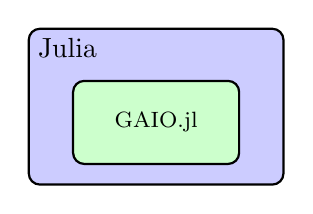
\begin{tikzpicture}[auto, node distance=2cm,>=latex']
    \node at (0,-2) [block] (julia) {\parbox{3cm}{Julia\vspace*{1.5cm}}};
    \node at (0,-2.2) [block,fill=green!20] (gaio) {{\footnotesize GAIO.jl}};
\end{tikzpicture}
    \caption{GAIO.jl architecture}
    \label{fig:arch}
\end{figure}

GAIO was fully redesigned and rebuilt in the Julia language starting in 2020. The reason to do so (and the decision to use Julia) was twofold:

\begin{enumerate}
    \item[Solving the two (or three\dots) language problem.] The cell mapping techniques require far too many function evaluations to be reasonable in an interpreted language. As with many scientific computing applications, compilation into fast machine code is necessary if one wishes to apply the methods to any real-scale problem. However, the primary userbase is mathematicians, not computer scientists. The code must therefore be easy to read, and it should be easy to convert pseudocode into usable software written in the style of a scripting language. Furthermore, the old software architecture had become difficult to maintain, even after being streamlined to just C and Matlab. 
    
    \item[No longer needing to tradeoff simplicity and transparency.] The speed of a modern compiled language on today's hardware comes with an added benefit: code does not \emph{need} to be hyper-optimized - "mostly" optimized is good enough. GAIO originally used a tree data structure to represent partitions of phase space in such a way that each box was represented by a precise bitstring, maximally utilizing every byte of memory. While this was efficient, it made the data difficult to decipher. More generally, a decision always had to be made. Either
    
    \begin{enumerate}
        \item complexity is hidden behind convenience functions, sacificing knowledge of "what's actually going on", or,
        \item code is "transparent", allowing for extensibility while sacrificing clarity. 
    \end{enumerate}

    GAIO.jl was written with the knowledge that today, this just is not strictly necessary anymore. A memory-efficient tree structure is still offered, but the primary technique for partitioning phase space is much simpler: just use a grid with Cartesian indices - \emph{keep it simple, stupid}. 
\end{enumerate}

\begin{figure}
\begin{lstlisting}[language=Matlab,mathescape]
function relative_attractor(tree, f, steps)
    for i = 1:steps,
        tree.set_flags('all', to_be_subdivided); 
        tree.subdivide(to_be_subdivided);   
        b = tree.boxes(-1); 
        while (~isempty(b))
            c = b(1:d); 
            r = b(d+1:2*d);
            P = X*diag(r) + ones(size(X))*diag(c); 
            tree.set_flags(f(P)$'$, hit);          
            b = tree.next_box(-1);
        end
        tree.remove(hit);                         
    end
\end{lstlisting}
\caption{Relative attractor algorithm in Matlab. Compare with Fig. \ref{fig:attr_julia}}
\label{fig:attr_matlab}
\end{figure}

\subsection{Fitting into Julia's active scientific computing ecosystem}

Another reason for the decision to use Julia for GAIO.jl is the large (and growing) open source scientific computing community. GAIO.jl makes extensive use of linear algebra routines (LinearAlgebra.jl \cite{bezanson2017julia}), sparse arrays (SparseArrays.jl \cite{bezanson2017julia}, Arpack.jl \cite{arpack}), graph/network routines (MatrixNetworks.jl \cite{matrixnetworks}), and numerical integrators (DifferentialEquations.jl \cite{differentialequations}), plotting ecosystems (Makie.jl \cite{makie}, Plots.jl \cite{plots}), among others. 

A particular example of the effectiveness of such an open source scientific computing model is CUDA.jl. The sample-point methods for cell mapping are examples of so-called \emph{embarrassingly parallel} \cite{parallel} problems. It has therefore been a long-standing desire to utilize the GPU to perform such massively parallel algorithms in GAIO. However, under the previous architecture this would have to be written in CUDA's native C interface, which suffers the issues mentioned in the preceeding section. 

This is solved by the amazing work done to create CUDA.jl. The cell mapping can be written as a generic kernel whose length (in lines of code) is the same as the standard code, meaning the algorithms that make up GAIO.jl can receive up to a 200-fold \cite{gaiocuda} performance boost without ever sacrificing readability. 

Furthermore, the open-source nature of Julia's scientific computing ecosystem has helped in programming GAIO.jl countless times. Since code is freely available, code reuse is common among the Julia community. Problems which have already been solved by other programmers need not be solved again. 

\section{Conclusion}

The Julia package GAIO.jl is introduced via an example of a three dimensional dynamical system. The software has been redesigned and rebuilt from the ground up to balance high performance and elegance, no longer needing to rely on two languages to do so. Future work is planned to use these structures e.g. for homology computation in cubical complexes, as well as to even more tightly integrate into the existing scientific computing ecosystem e.g. DynamicalSystems.jl \cite{dynamicalsystemsjl,dynamicalsystemsbook} in the Julia programming language. 

\input{bib.tex}

\end{document}

% Inspired by the International Journal of Computer Applications template
